\chapter{Tribal NeuroSim: a szimuláció alapjai és felépítése}

\section{Célkitűzés és kutatási kapcsolat}

A Tribal NeuroSim a PremadeGraph gráfelemzési pipeline közvetlen folytatása. A PremadeGraph pipeline minden egyes játékosklasztert teljesítménymetrikák halmazával jellemez: harci hatékonyság, erőforrás-gazdálkodás, objektívkontroll, kockázattűrés és csapatkoordináció. Ezek az értékek aggregált klaszterszintű mérőszámokká állnak össze (\textit{A\_combat}, \textit{A\_resource}, \textit{A\_map\_objective}, \textit{A\_risk}, \textit{A\_team}), amelyek a Tribal NeuroSim törzseinek iniciális genomszekvenciáját alkotják.

A szimulációban egyidejűleg mindkét adatkészlet klaszterei megjelennek. A kutatási kérdés: ha Flex Queue-ból és SoloQ-ból derivált klaszterprofilok azonos szimulációs szabályrendszer alatt versenyeznek, vajon a mögöttes gráfstruktúra mérhető különbséget idéz-e elő az emergáló túlélési stratégiákban?

A kísérlet kerete exploratív transzfer-vizsgálat \cite{bonabeau2002}. Nem kísérel meg közvetlen előrejelzést valódi meccskimenetelekre, és nem állít fel pszichológiai vagy szociológiai kauzalitást.

\section{Ágensorientált és többügynök-modell}

A Tribal NeuroSim ágensorientált modell (ABM): minden törzs önálló döntéshozó egység, amely kizárólag saját lokális állapota és közvetlen térbeli környezete alapján cselekszik. A makroszintű minták (terjeszkedés, háborúk, birodalomkialakulás, kihalás) kizárólag az egyéni döntések összegzéseként jelennek meg \cite{bonabeau2002}.

A rendszer többügynök-rendszerként (MAS) is értelmezhető \cite{wooldridgejennings1995}: minden törzs önálló ágensként működik saját belső állapottal, saját lokális percepcióval és saját döntési logikával (neurális hálózat). Az ágensek között nincs közvetlen kommunikáció: interakció kizárólag a közös térbeli szubsztráton keresztül zajlik.

A szimuláció lefolyása azonos szerkezetű fázisokat mutat: korai terjeszkedés (tick~0-300), konszolidáció (tick~300-1000), majd birodalmi háborúk (tick~1000+).

\section{A rendszer felépítése}

\begin{figure}[H]
\centering
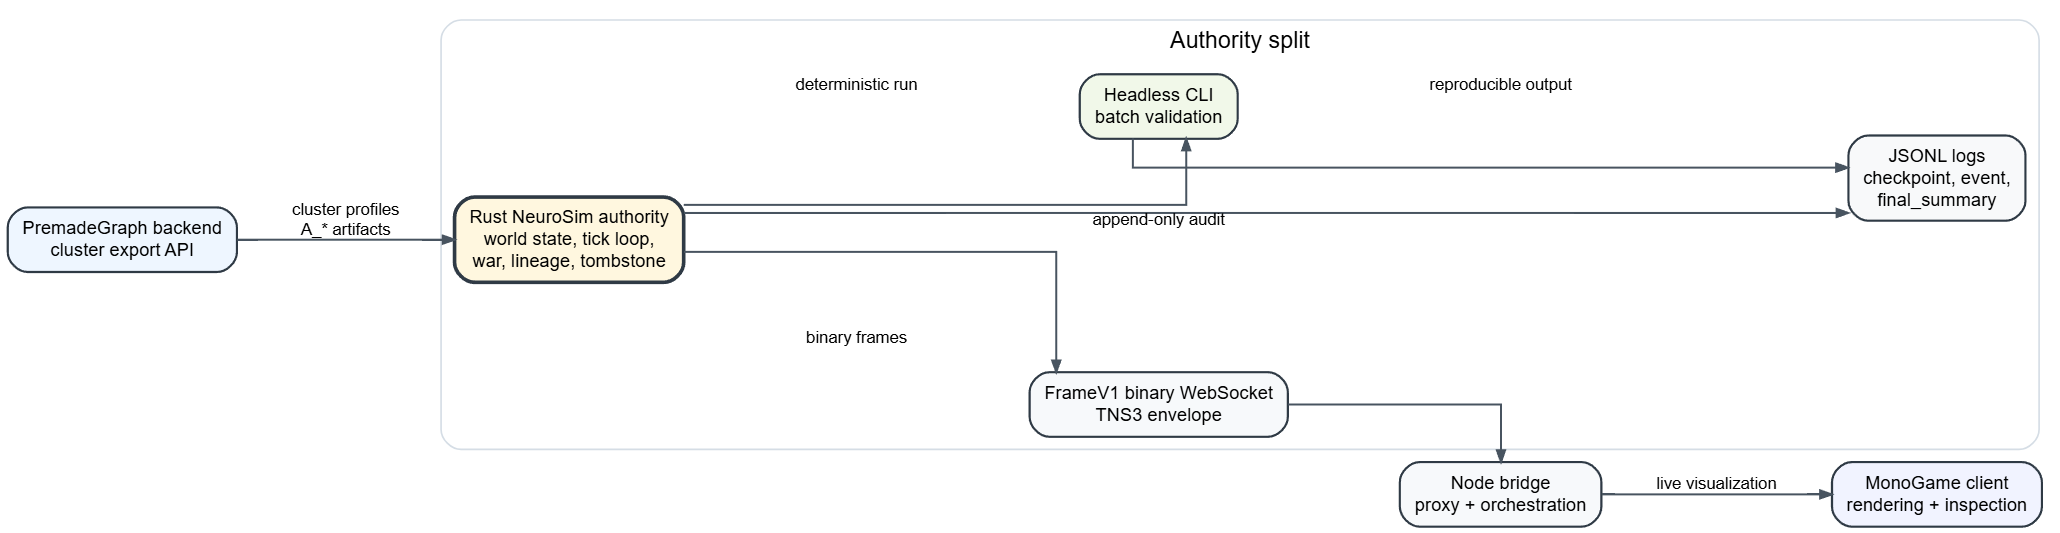
\includegraphics[width=0.92\textwidth]{assets/diagrams/thesis_neurosim_architecture_graphviz.png}
\caption{A Tribal NeuroSim hatáskör-megosztása: a Rust motor az autoritatív szimulációs állapot forrása, míg a Node és MonoGame rétegek közvetítő és megjelenítő szerepet kapnak.}
\label{fig:neurosim-architecture-graphviz}
\end{figure}

A \textbf{Rust futtatókörnyezet} az autoritás egyetlen forrása: a tick-ciklust, a világállapotot, a törzsek neurális döntéshozatalát, a háború- és szövetségfeloldást, a fuzionálási logikát, a tombstone-bejegyzéseket és az eseménynaplózást mind a Rust bináris kezeli \cite{jung2020}. A \textbf{C\# MonoGame kliens} kizárólag vizualizáció és operátori felület. A \textbf{Node réteg} vékony közvetítő: összekötőhíd a MonoGame és a Rust szerver között.

Ez a felosztás a böngészőalapú v2 prototípus közvetlen tanulsága: ahol a szimulációs állapot az UI-réteghez volt csatolva, ghost war jelenség, memóriaszivárgás és nem-determinisztikus viselkedés keletkezett.

A ghost war konkrétan azt jelentette, hogy két törzs egyidejűleg különböző háborús állapotot észlelt: az egyik már befejezettnek tekintette az összecsapást, a másik még folyamatban lévőként kezelte. Az ok az volt, hogy az UI tartotta a szimulációs állapotot, és HTTP-kérések között az állapot szétcsúszhatott. A jelenlegi architektúrában minden döntés a Rust binárisban születik; a MonoGame kliens csak a legutóbb kapott frame-et rendereli, így nincs szétcsúszás, és a szimuláció bármely pillanatban reprodukálható ugyanabból a kezdőállapotból.

\section{FrameV1 bináris protokoll}

A Rust szerver és a MonoGame kliens bináris WebSocket kereteken kommunikál. Minden keret egy 40 bájtos \textit{TNS3} envelope-pal kezdődik (little-endian):

\begin{table}[H]
\centering
\caption{FrameV1 desktop envelope fejléc.}
\label{tab:framev1-envelope}
\begin{tabular}{|r|l|l|}
\hline
\textbf{Offset} & \textbf{Méret} & \textbf{Mező} \\
\hline
0  & 4 B & Magic: \textit{"TNS3"} \\
4  & 2 B & Version: \textit{1} \\
6  & 2 B & HeaderBytes: \textit{40} \\
8  & 2 B & PayloadKind: \textit{2} (\textit{FrameV1}) \\
10 & 2 B & Flags \\
12 & 4 B & PayloadBytes \\
16 & 8 B & Tick (\textit{u64}) \\
24 & 4 B & Generation (\textit{u32}) \\
28 & 4 B & RecordCount (élő törzsek száma) \\
32+ & változó & V1 payload \\
\hline
\end{tabular}
\end{table}

A bináris formátum döntése teljesítményi: a Rust szerver 40~ms alatt lekezel 599 törzs állapotát, miközben a MonoGame kliens aszinkron dekódol és renderel. A JSON sorosítás elkerülése egy 599-törzsös világ esetén tick-enként ~150--200~kB felesleges szöveges overhead-et spórol meg.

Az eseményvezérelt megfigyelhetőség részletei és a determinizmus-hiba javítása (\textit{clusters.sort\_by(|a, b| a.id.cmp(\&b.id))}) a kibővített verzió 13. fejezetében találhatók \cite{premadegraph-full}.
